% 第 17 题仓库组合体图（正四棱柱 + 正四棱锥，本项目首例组合体）：按固定源 PDF 矢量路径换算（1 pt → 0.03515 cm）。
% 原点取 A 点（源页 (1033.48, 292.36) pt），y 向上。
% 下部正四棱柱 ABCD-A₁B₁C₁D₁（斜二测，前表面与右表面可见）；
% 上部正四棱锥 P-A₁B₁C₁D₁（叠在顶面上，四条侧棱均实线）。
% 实线 12 段（棱锥 4 侧棱 + 顶面前/右/左 3 棱 + 底面可见棱 + 3 条可见侧棱）；
% 虚线 5 段（被遮挡的 AD/DC/DD₁/C₁D₁ + 竖直中轴虚线 O–O₁–P 一条，串联两高的共线关系）。
% O、O₁ 处实心点（源内标签在左、点在右）；照源复刻。
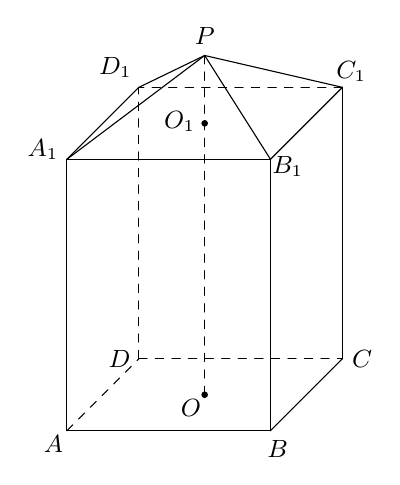
\begin{tikzpicture}[line cap=round,line join=round,font=\small,x=0.03515cm,y=0.03515cm]
% ===== 实线（12 段）=====
\draw (49.76,135.54)--(0,98.04);       % P–A₁
\draw (49.76,135.54)--(73.53,98.04);   % P–B₁
\draw (49.76,135.54)--(99.52,124.03);  % P–C₁
\draw (49.76,135.54)--(25.99,124.03);  % P–D₁
\draw (0,98.04)--(73.53,98.04);        % A₁–B₁（顶面前棱）
\draw (73.53,98.04)--(99.52,124.03);   % B₁–C₁（顶面右棱）
\draw (25.99,124.03)--(0,98.04);       % D₁–A₁（顶面左棱）
\draw (0,0)--(73.53,0);                % A–B（底面前棱）
\draw (73.53,0)--(99.52,25.99);        % B–C（底面右棱）
\draw (0,0)--(0,98.04);                % A–A₁（前左侧棱）
\draw (73.53,0)--(73.53,98.04);        % B–B₁（前右侧棱）
\draw (99.52,25.99)--(99.52,124.03);   % C–C₁（后右侧棱）
% ===== 虚线（5 段）=====
\draw[dash pattern=on 2.99pt off 2.99pt] (0,0)--(25.99,25.99);         % A–D
\draw[dash pattern=on 2.99pt off 2.99pt] (25.99,25.99)--(99.52,25.99); % D–C
\draw[dash pattern=on 2.99pt off 2.99pt] (25.99,25.99)--(25.99,124.03); % D–D₁
\draw[dash pattern=on 2.99pt off 2.99pt] (99.52,124.03)--(25.99,124.03); % C₁–D₁
\draw[dash pattern=on 2.99pt off 2.99pt] (49.76,12.99)--(49.76,135.54); % O–O₁–P（两高共线）
% ===== 实心点（O、O₁ 处）=====
\fill (49.76,12.99) circle (1.2pt);
\fill (49.76,111.03) circle (1.2pt);
% ===== 标注（照源字框中心，显式坐标；O/O₁ 标签在点之左）=====
\node[anchor=center,inner sep=0] at (49.83,142.51) {\(P\)};
\node[anchor=center,inner sep=0] at (17.51,131.15) {\(D_{1}\)};
\node[anchor=center,inner sep=0] at (102.73,129.75) {\(C_{1}\)};
\node[anchor=center,inner sep=0] at (-8.63,101.66) {\(A_{1}\)};
\node[anchor=center,inner sep=0] at (79.78,95.39) {\(B_{1}\)};
\node[anchor=center,inner sep=0] at (18.96,25.98) {\(D\)};
\node[anchor=center,inner sep=0] at (106.63,25.99) {\(C\)};
\node[anchor=center,inner sep=0] at (-4.89,-4.76) {\(A\)};
\node[anchor=center,inner sep=0] at (76.14,-6.45) {\(B\)};
\node[anchor=center,inner sep=0] at (40.70,111.82) {\(O_{1}\)};
\node[anchor=center,inner sep=0] at (44.83,8.06) {\(O\)};
\end{tikzpicture}
